% !TeX spellcheck = en_US
\addsection{Resources}{\skills/estates.png}

\begin{multicols}{2}

\hypertarget{Resources}{There}\index{Resources} are three types of Resources in the game: Gold \includesvg[height=10px]{\svgs/gold.svg}, Building Materials \includesvg[height=10px]{\svgs/building_materials.svg}, and Valuables \includesvg[height=10px]{\svgs/valuablegreater.svg}.
Resources are spent during the game to expand your \hyperlink{Town}{Town}, to Recruit \hyperlink{Units}{Units}, and to purchase \hyperlink{spells}{Spells}.
You can gain Resources from the \hyperlink{Mines}{Settlements and Mines} that you have \hyperlink{Categories}{Flagged}, and also by playing Cards and rolling Resource Dice \includesvg[height=10px]{\svgs/resource_die.svg}.
Whenever a player's Resource Production is increased or decreased, move that Resource's cube on its production track the appropriate number of spaces.\par
\begin{multicols}{3}
  \centering
  \vspace*{\fill}
  
\includegraphics[width=0.8\linewidth]{\images/gold.png}
  \footnotesize\textcolor{darkcandyapplered}{\textit{\textbf{Gold \phantom{Materials}}}}
  \columnbreak
  \vspace*{\fill}
  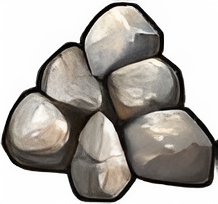
\includegraphics[width=0.8\linewidth]{\images/building_materials.png}
  \footnotesize\textcolor{darkcandyapplered}{\textit{\textbf{Building Materials}}}
  \columnbreak
  \vspace*{\fill}
  
\includegraphics[width=0.8\linewidth]{\images/valuables.png}
  \footnotesize\textcolor{darkcandyapplered}{\textit{\textbf{Valuables \phantom{Materials}}}}
\end{multicols}
Players start each Scenario with the number of Resources indicated in that Scenario’s setup.
Resources can also be \hyperlink{Trading}{traded}.
There's no limit to the amount of Resources you can have.

\vspace*{\fill}

\columnbreak

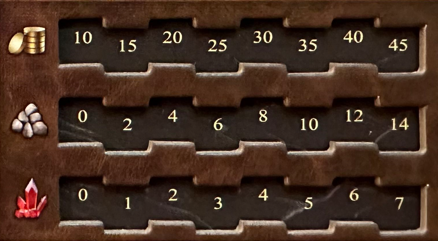
\includegraphics[width=\linewidth]{\tables/resource_board.png}
\smallskip
\centering\footnotesize\textcolor{darkcandyapplered}{\textbf{\textit{Resource Production Tracker}}}
\bigskip

Possible Resource Die\index{Resource Die}\index{Dice} \includesvg[height=10px]{\svgs/resource_die.svg} results:
\medskip
\begin{itemize}
  \setlength\itemsep{8pt}
  \item \includesvg[height=15px]{\svgs/2_building_materials.svg} - 2 x Building Materials
  \item \includesvg[height=15px]{\svgs/4_building_materials.svg} - 4 x Building Materials
  \item \includesvg[height=15px]{\svgs/1_valuables.svg} - 1 x Valuables
  \item \includesvg[height=15px]{\svgs/2_valuables.svg} - 2 x Valuables
  \item \includesvg[height=15px]{\svgs/3_gold.svg} 3 x Gold
  \item \includesvg[height=15px]{\svgs/6_gold.svg} 6 x Gold
\end{itemize}

\begin{tikzpicture}[overlay]
  \node at (2, 1.5) {
\includegraphics[width=0.3\linewidth]{\images/resource_die.png}};
\end{tikzpicture}

\end{multicols}

\vspace*{\fill}

\begin{scaledfigure}[blanker]
  \centering
  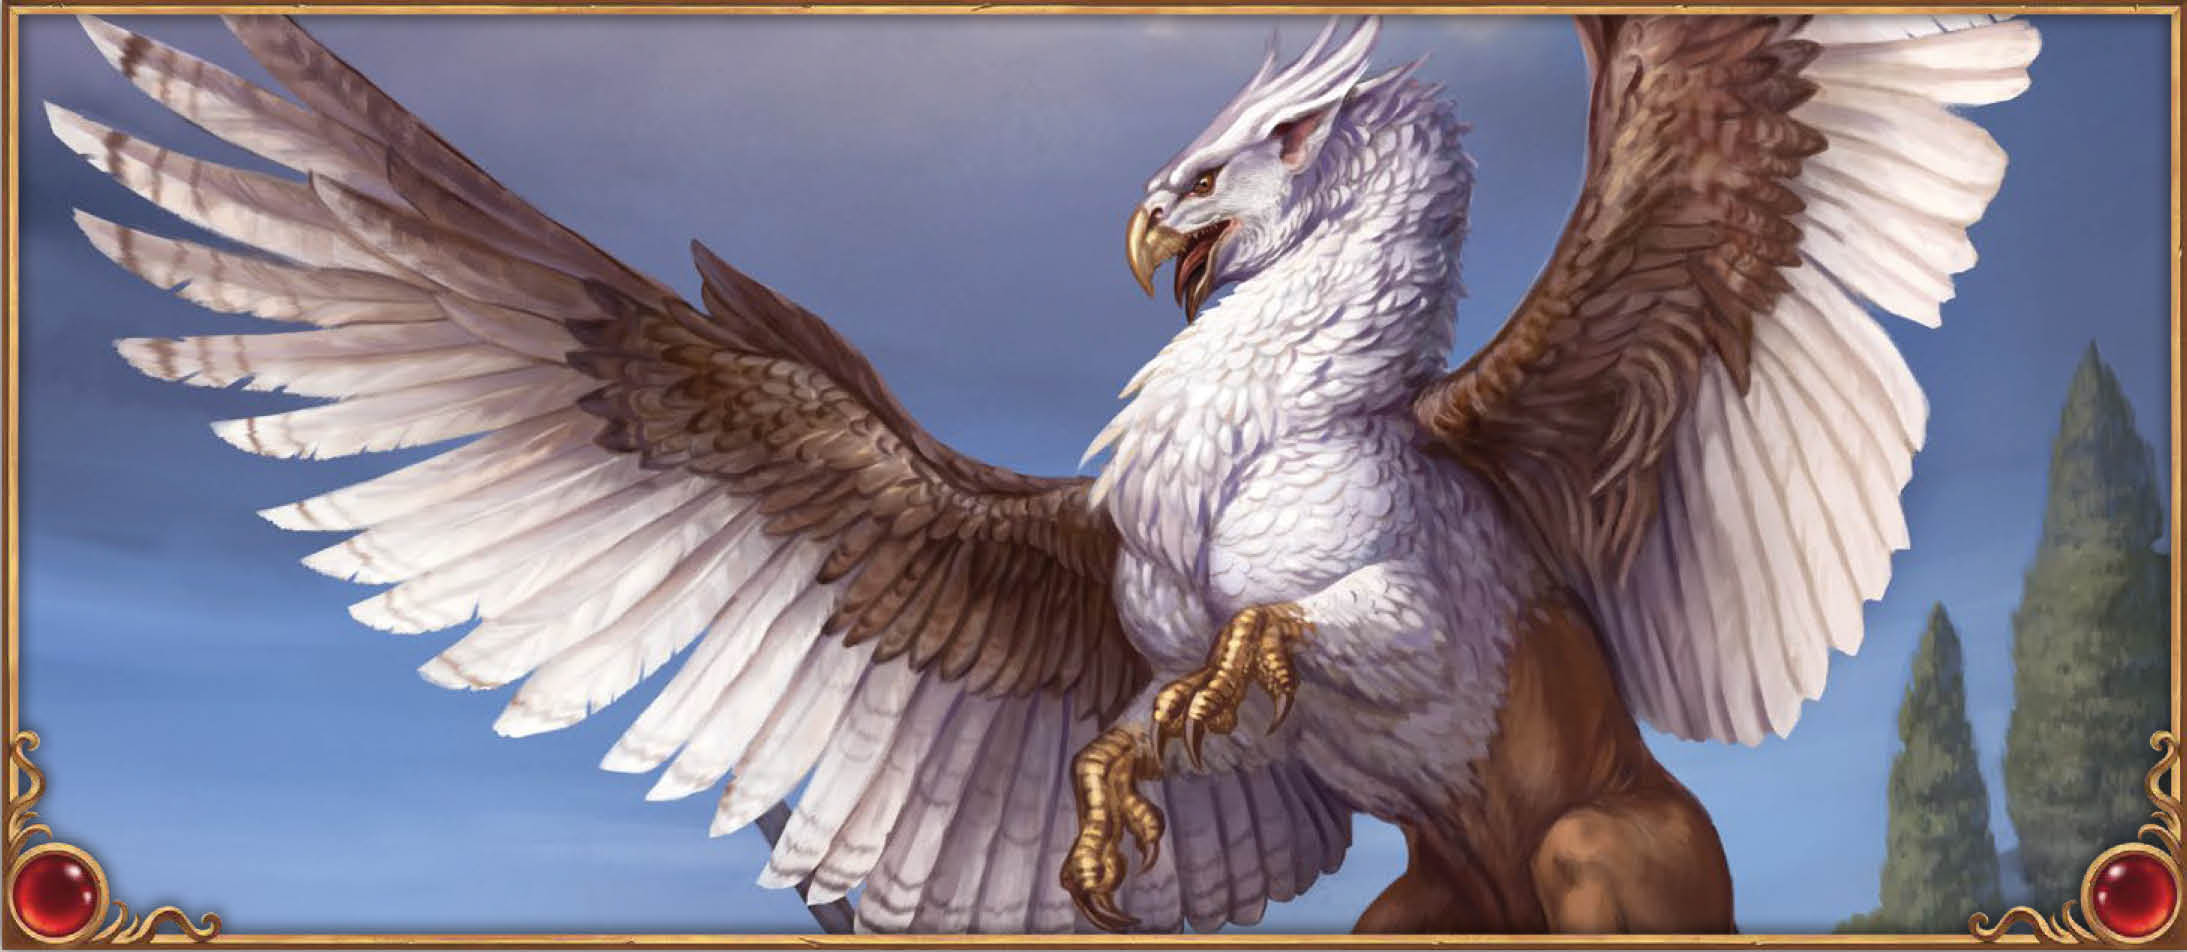
\includegraphics[width=\linewidth, height=\myspace, keepaspectratio]{\art/griffin.jpg}
\end{scaledfigure}
